\phantomsection
\section*{6 线性映射矩阵表示}
\addcontentsline{toc}{section}{6 线性映射矩阵表示}

\vspace{2ex}

\centerline{\heiti A组}
\begin{enumerate}
    \item
\end{enumerate}

\centerline{\heiti B组}
\begin{enumerate}

    \item 证明:\begin{enumerate}
              \item 由于 $ \ker \sigma = \im \sigma $,由 $ \dim \im \sigma + \dim \ker \sigma = \dim V $ 可得.

              \item 设 $ \beta_1, \ldots, \beta_n $ 为 $ V $ 的一组基,则
                    \[ \im \sigma = \spa(\sigma(\beta_1), \ldots, \sigma(\beta_n)) = \ker \sigma \]
                    设 $ \sigma(\beta_1), \ldots, \sigma(\beta_{\frac{n}{2}}) $ 为 $ \im \sigma $ 的基,则可以证明
                    \[ \sigma(\beta_1), \ldots, \sigma(\beta_{\frac{n}{2}}), \beta_1, \ldots, \beta_{\frac{n}{2}} \]
                    线性无关,且 $ \sigma $ 在此基下的矩阵即为所求的形式.
          \end{enumerate}

\end{enumerate}

\centerline{\heiti C组}
\begin{enumerate}
    \item 证明:必要性:$ \forall \alpha \in V $,由 $ \sigma $ 可逆,存在唯一的 $ \beta \in V $ 使得 $ \sigma(\beta) = \alpha $ 且 $ \beta = \beta_1 + \beta_2 $,其中 $ \beta_1 \in W_1 $,$ \beta_2 \in W_2 $. 于是
          \[ \alpha = \sigma(\beta) = \sigma(\beta_1) + \sigma(\beta_2) \in \sigma(W_1) + \sigma(W_2) \]
          所以 $ V \subseteq \sigma(W_1) + \sigma(W_2) $.

          $ \sigma(W_1), \sigma(W_2) $ 都是 $ V $ 的子空间,它们的和也是 $ V $ 的子空间. 所以 $ \sigma(W_1) + \sigma(W_2) \subseteq V $,故 $ V = \sigma(W_1) + \sigma(W_2) $.

          充分性:$ \forall \alpha \in V = \sigma(W_1) + \sigma(W_2) $,$ \exists \alpha_i \in \sigma(W_i) $ 且 $ \exists \beta_i \in W_i $ 使 $ \alpha_i = \sigma(\beta_i) $($ i = 1, 2 $)使得
          \[ \alpha = \alpha_1 + \alpha_2 = \sigma(\beta_1) + \sigma(\beta_2) = \sigma(\beta_1 + \beta_2) = \sigma(\beta) \]
          其中 $ \beta = \beta_1 + \beta_2 \in W_1 + W_2 = V $,所以 $ \sigma $ 为满射.

          由于 $ n $ 维线性空间上的线性映射为满射时也必为单射,从而必是双射,所以 $ \sigma $ 可逆.

    \item 证明:先证右边. 由于 $ \sigma(V_1) \subseteq V_2 $,所以 $ (\tau \sigma)(V_1) \subseteq \tau(V_2) $,如下图所示. 因此
          \[ \dim(\tau \sigma)(V_1) \leqslant \dim \tau(V_2) \]
          即 $ r(\tau \sigma) \leqslant r(\tau) $.
          \begin{figure}[H]
              \centering
              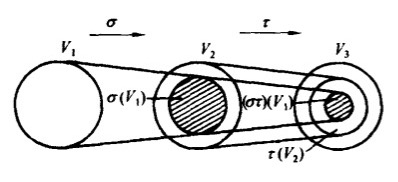
\includegraphics[scale=.5]{figs/6C.2.1.jpg}
          \end{figure}
          又因为 $ (\tau \sigma)(V_1) = \tau(\sigma(V_1)) $,所以又有
          \[ \dim(\tau \sigma)(V_1) \leqslant \dim \sigma(V_1) \]
          即 $ r(\tau \sigma) \leqslant r(\sigma) $.

          再证左边. 由线性映射维数公式,
          \begin{gather*}
              r(\tau) + \dim \ker \tau = n \\
              r(\tau \sigma) + \dim \ker(\tau \sigma) = m
          \end{gather*}
          又 $ \dim \ker(\tau \sigma) \leqslant \dim \ker \tau $,所以
          \[ m - r(\tau \sigma) = \dim \ker(\tau \sigma) \leqslant \dim \ker \tau \]
          代入线性映射维数公式,得 $ \dim \ker \tau = n - r(\tau) \geqslant m - r(\sigma) $,即
          \begin{align*}
              r(\tau \sigma) & \geqslant m + r(\tau) - n         \\
                             & \geqslant r(\sigma) + r(\tau) - n
          \end{align*}

    \item 证明:由于 $ \forall \beta \in (\sigma + \tau)(V_1),\enspace \exists \alpha \in V_1 $ 使 $ \beta = (\sigma + \tau)(\alpha) = \sigma(\alpha) + \tau(\alpha) \in \sigma(V_1) + \tau(V_1) $,所以
          \[ (\sigma + \tau)(V_1) \subseteq \sigma(V_1) + \tau(V_1) \]
          因此
          \begin{align*}
              \dim(\sigma + \tau)(V_1) & \leqslant \dim(\sigma(V_1) + \tau(V_1))     \\
                                       & \leqslant \dim \sigma(V_1) + \dim \tau(V_1)
          \end{align*}

    \item 证明:\begin{enumerate}
              \item \label{item:6:C:4:1}
                    $ \forall \sigma \in \mathcal{L}(V, V) $,则 $ I - \sigma \in \mathcal{L}(V, V) $. $ \forall \alpha \in (I - \sigma)(V),\enspace \exists \beta \in V $,有
                    \begin{gather*}
                        \alpha = (I - \sigma)(\beta) = \beta - \sigma(\beta) \\
                        \sigma(\alpha) = \sigma(\beta - \sigma(\beta)) = \sigma(\beta) - \sigma^2(\beta)
                    \end{gather*}
                    而由于 $ \sigma^2 = \sigma $,所以 $ \sigma(\alpha) = \vec{0} $,于是 $ \alpha \in \ker \sigma $,因此 $ (I - \sigma)(V) \subseteq \ker \sigma $.

              \item 利用 $ r(\sigma + \tau) \leqslant r(\sigma) + r(\tau) $ 和 $ r(\sigma) + \dim \ker \sigma = n $,由 \ref*{item:6:C:4:1} 可得
                    \begin{equation} \label{eq:6:C:4:2:1}
                        r(I - \sigma) + r(\sigma) \leqslant n
                    \end{equation}
                    又因为
                    \begin{equation} \label{eq:6:C:4:2:2}
                        r(I - \sigma) + r(\sigma) \geqslant r(I - \sigma + \sigma) = r(I) = n
                    \end{equation}
                    于是由\autoref{eq:6:C:4:2:1} 和\autoref{eq:6:C:4:2:2} 即可得到 $ r(I - \sigma) + r(\sigma) = n $.
          \end{enumerate}

    \item 证明:\begin{enumerate}
              \item \label{item:6:C:5:1}
                    $ \forall \alpha \in \im \sigma,\enspace \exists \beta \in V $ 使得 $ \sigma(\beta) = \alpha $. 由 $ \sigma^2 = \theta $ 可得 $ \sigma(\alpha) = \sigma^2(\beta) = \vec{0} $,因此 $ \alpha \in \ker \sigma $,从而 $ \im \sigma \subseteq \ker \sigma $. 于是我们得到
                    \[ n = \dim \im \sigma + \dim \ker \sigma \geqslant 2 \dim \im \sigma \]
                    即 $ \dim \im \sigma \leqslant \dfrac{n}{2} $.

              \item 由 \ref*{item:6:C:5:1} 可知,方程组 $ AX = \vec{0} $ 的基础解系含有 $ n - r(A) = \dim \ker \sigma \geqslant \dfrac{n}{2} $ 个解向量,所以结论成立.
          \end{enumerate}

    \item 假设 $ \alpha_1, \alpha_2, \ldots, \alpha_n \in \mathbf{F} $ 是 $ \mathbf{F} $ 作为数域 $ \mathbf{K} $ 上的线性空间的一组基,$ \beta_1, \ldots, \beta_m \in \mathbf{E} $ 是 $ \mathbf{E} $ 作为数域 $ \mathbf{F} $ 上的线性空间的一组基,则现在对于任意的 $ \beta \in \mathbf{E} $,都存在 $ k_1, \ldots, k_m \in \mathbf{F} $ 使得 $ \beta = \displaystyle\sum_{i = 1}^{m} k_i \beta_i $.

          而对于每一个 $ k_i \in \mathbf{F},\enspace i = 1, 2, \ldots, m $,存在 $ l_{ij} \in \mathbf{K},\enspace j = 1, 2, \ldots, n $ 使得 $ k_i = \displaystyle\sum_{j = 1}^{n} l_{ij} a_j $. 于是
          \[ \beta = \sum_{i = 1}^{m} \sum_{j = 1}^{n} l_{ij} \alpha_j \beta_i \]
          这说明对任意的 $ \beta \in \mathbf{E} $,都可由
          \[ \alpha_1 \beta_1, \ldots, \alpha_1 \beta_m, \alpha_2 \beta_1, \ldots, \alpha_n \beta_m \]
          这 $ mn $ 个向量线性表出,其中线性表出的系数都属于最小的数域 $ \mathbf{K} $.

          同时,如果假设 $ l_{ij} \in \mathbf{K} $ 满足 $ \displaystyle\sum_{i = 1}^{m} \sum_{j = 1}^{n} l_{ij} \alpha_j \beta_i = 0 $,则
          \[ \sum_{i = 1}^{m} \left(\sum_{j = 1}^{n} l_{ij} \alpha_j\right) \beta_i = 0 \]
          利用 $ \beta_1, \ldots, \beta_m $ 的线性无关性可得 $ \displaystyle\sum_{j = 1}^{n} l_{ij} \alpha_j = 0 $,再结合 $ \alpha_1, \ldots, \alpha_n $ 线性无关可得 $ l_{ij} = 0 $,这就说明 $ \alpha_1 \beta_1, \ldots, \alpha_1 \beta_m, \alpha_2 \beta_1, \ldots, \alpha_n \beta_m $ 在数域 $ \mathbf{K} $ 是线性无关的.

          综上,$ \alpha_1 \beta_1, \ldots, \alpha_1 \beta_m, \alpha_2 \beta_1, \ldots, \alpha_n \beta_m $ 就是 $ \mathbf{E} $ 作为 $ \mathbf{K} $ 的线性空间的一组基,从而这个线性空间是 $ mn $ 维的.
\end{enumerate}

\clearpage
